%! Author = User
%! Date = 13.09.2023

% Preamble
\documentclass[a4paper,10pt,twocolumn]{article}

% Packages 
\usepackage[utf8]{inputenc}  %man kann Sonderzeiche wie ü,ö usw direkt eingeben
\usepackage{amsmath}           %macht
\usepackage{amsfonts}          %       Mathe
\usepackage{amssymb}           %              mächtiger
\usepackage{graphicx}          %erlaubt Graphiken einzubinden (.eps für dvi und ps sowie .jpg für pdf)
\usepackage[T1]{fontenc}       %Zeichenbelegung der verwendeten Schrift
\usepackage{ae}                %macht schöneres ß
\usepackage{typearea}
\usepackage{amstex}
\usepackage{siunitx}
\usepackage{hyperref}	         %ermöglicht änderung des Seitenspiegels


\usepackage{amsmath}
\usepackage{tikz}
\usepackage{pgfplots}

\newcommand{\alphaNoError}{(4.047 \pm 0.036)}
\newcommand{\betaNoError}{(-4.73 \pm 0.29) \cdot 10^{-3}}
\newcommand{\halfTimeNoError}{(146.5 \pm 9.1)\ s}
\newcommand{\alphaGauss}{(4.04 \pm 0.10)}
\newcommand{\betaGauss}{(-4.62 \pm 0.95) \cdot 10^{-3}}
\newcommand{\halfTimeGauss}{(150 \pm 31)\ s}
\newcommand{\alphaPoisson}{(4.05 \pm 0.10)}
\newcommand{\betaPoisson}{(-4.75 \pm 0.95) \cdot 10^{-3}}
\newcommand{\halfTimePoisson}{(146 \pm 29)\ s}
\newcommand{\symN}{\delta N}



\pagestyle{scrheadings}        %sagt Koma-Skript, dass selbstdefiniers Kopfzeilen verwendet werden
\typearea{16}                  %stellt Seitenspiegel ein
\columnsep25pt								 %definiert Breite zwischen den zwei Spalten von \twocolumns

\renewcommand{\pnumfont}{%     %ändert die Schriftart der Seitennummerierung
    \normalfont\rmfamily\slshape}  %ändert die Schriftart der Seitennummerierung 



\begin{document}
    \twocolumn[{\csname @twocolumnfalse\endcsname                %erlaubt "Abstrakt" über beide Spalten
    \titlehead{                                                  %Kopfzeile
        \begin{tabular*}{\textwidth}[]{@{\extracolsep{\fill}}lr}   %Kopfzeile
            Betreuer: Ronny Thomale & \today\\                          %Kopfzeile - Betreuer
        \end{tabular*}                                             %Kopfzeile
    }
    \title{Experimental methods for examining properties of classical light with microwaves and using bragg reflection to examin cirstal structur}  %Titel der Versuchs
    \author{Salahudin Smailagić and Thomas Karb}                     %Namen der Studenten
    \date{}                                                         %benötigt um automatisches Datum auszuschalten
    \maketitle                                                      %erzeugt Titelseite
    \vspace{-5ex}                                                   %verringert Abstand zur Überschrift
    \begin{abstract}                                                %Beginn des Abstracts
        We used experiments with microwaves to show the wave character of light.
        Via inteference we determined the wavelenght of the microwaves. 
        \\
        Measuerement made: 19. September 2023\\       %Datum ändern!
        Submitted: 26. September 2023                %Datum ändern!
        \\
        \\
    \end{abstract}
    }]
    \section{Introduction}
    To study the classical wave-properties of light we use microwaves, since they have a large wave lenght in the cm-range.
    Effects like interference and tunneling occur on a macroscopic scale with microwaves, which makes it easy to show them
    in an experiment.
    Because all properties showed here with microwaves apply also for light in the visible spectrum, you can use 
    reuse our results, but on a different scale of length.
    \section{Experimental setup}
    \subsection{Emitter}
    A Gunn diode was used to create the microwaves in our experiments. 
    It has a horn antenna for focusing the light.
    We measured the angle-intensity relation and made a basic gauss-fit to get a rough estimate of the light dispersion (cf.~\ref{fig:AngleDispersion}).
    The full-width-half-maximum of the used emitter is
    \begin{align*}
        fwhm = \AngleDispersionGaussFWHM
    \end{align*}

    \figAngleDispersion{caption angle dispersion}


    \subsection{Lens}
    For the experiments with bragg reflection and tunnel effect we need parallel light rays.
    We used a wax lens for focusing the emitted microwaves.
    To determine the focal length the lens was placed in away from the emitting diode.
    The effective object (emitter) distance after~\cite{pasco} in our setup was $g = \ObjectDistance$
    Then for varying receiver positions the intensity was measured as shown in~\ref{fig:imageDistance}. 
    Because the wavelength is in the cm range, the diameter of the resulting airy disk is also in the cm range.
    This means there is no distance were the object (emitter) is completely focused as you would expect from geometric optics.
    So to access the image distance we made a gauss-fit over the intensity distribution and used the maximum of the fit as
    reference. 
    \figimageDistance{caption image Distance}
    Here $b = \ImageDistance$

    Now we can calculate the focal length after the lens formula
    \begin{align*}
        \frac{1}{f} = \frac{1}{b} + \frac{1}{g}
    \end{align*}
    We have determined the focal length of the lens in our setup as:
    \begin{align*}
        f = \FocalLength
    \end{align*}
    \section{Wavelength measurement}
    It is important to know the wavelength of the light for the subsequent experiments.
    The wavelength by the manufacturer of the diode is
    \begin{align*}
        \lambda = \OfficialWaveLength
    \end{align*}
    To verify this we used to setups.
    \subsection{Stationary wave}
    For the first approach we create stationary waves.
    We position a mirror opposite of the emitter in a distance of $1m$.
    Then we move the receiver between mirror and diode and count the nodes of the resulting standing wave.
    We then measure the distance around 40 nodes and can calculate the wavelength:
    \begin{align*}
        \lambda = \StandingWavesWaveLength
    \end{align*}
    \subsection{Michelson interferometer}
    As the second approach we use an interferometer.
    The emitted light is split by a fiberboard as semi-transparent mirror in two perpendicular rays.
    Which then are reflected by two metal sheets and reunited again by the fiberboard. 
    In the resulting ray interferes constructive or destructive depending on the difference between the two optical paths
    and the wavelength.
    We move the position of one mirror and after seeing 10 maxima and minima on the detector we calculate the the changed
    path length.
    With our setup we have determined the wavelength as:
    \begin{align*}
        \lambda = \InterferometerWaveLength
    \end{align*}
    \begin{figure}[htbp]
        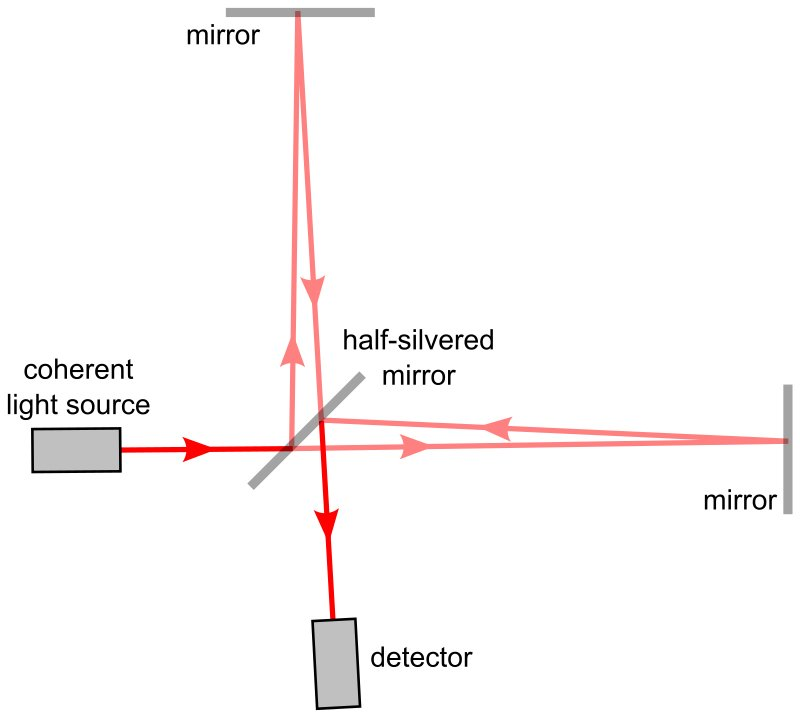
\includegraphics[width=0.9\linewidth]{Interferometer}
        \center
        \caption{By varing the optical path length of the rays you see constructive or destructive interference on the
        detector. This depends on the wavelength of the ligth, so you can use the method to measure the wavelength.
        Graphic from~\cite{imageMichelsonInterferometerWiki}}
        \label{fig:Interferometer}
    \end{figure}
    \section{Polarisation}
    The Gunn diode with the horn antenna in our setup emits vertical polarized light.
    Also the receiver detects in default configuration only vertical polarized light.
    This can be easily shown by rotating the receiver $ 90\degree$.
    Now no signal is being detected.
    If you then insert a linear polarisation filter in a $ 45\degree$ angle you will detect a signal.
    This follows because the vertical polarized E-field is projected on the polarisation filter.
    For the polarisation filter a simple metal grid was used with five lattice bars.

    As a quantitative assertion we arranged the receiver and emitter in vertical position and rotated the polarisation
    filter in an $ 180\degree $-arc and measured the angle-intensity distribution.
    Following malus's law the intensity after the filter is:
    \begin{align*}
        I = I_0 \cos^2(\phi)
    \end{align*}
    Since the metal grid and the receiver act as two polarisation filter our signal should follow the formula:
    \begin{align*}
        I = I_0 \cos^4( \phi )
    \end{align*}
    If we fit the function $U(\phi) = a + b \cos^4(\phi)$ to correct for the fact that we do not now the exact calibration 
    of the receiver, we still a strong deviation from the theoretical relationship.
    The reduced chi-square of the fit is:
    \begin{align*}
        \chi_{\nu}^2 = \PolarisationFitReducedResidual
    \end{align*}
    The deviation is probably due to the low number of lattice bars, which makes the polarisation filter not ideal.
    \figPolarisation{caption polarisation}
    \section{Total inner reflection and tunnel effect}
    An important property of light we were able to verify is total reflection and evanescent wave.
    For the experiment we emitted microwaves on a paraffin wax prism. 
    On the $45\degree$ paraffin-air boundary the rays are totally reflected and we detect them in an $90\degree$ rotated
    angle. 
    After the paraffin-air boundary an evanescent wave is formed.
    Its intensity declines exponentially.
    \begin{align*}
        I \propto e^{\frac{-2z}{s}} 
    \end{align*}
    Here z is the perpendicular distance and s is the declination rate which depends on the wavelength, 
    the angle of reflection and the refractive index.

    You can detect the evanescent wave by a adding a second prism after the $ 45\degree$ boundary parallel to the first one
    in the distance $z$.
    Now analogous to the quantenmechanical tunnel effect the light can propagate through the air gap and a signal can be
    detected.
    We have measured the reflected and transmitted microwaves for different gap sizes $z$ and then applied an exponential 
    fit as you can see in~\ref{fig:TotalReflection}

    \figTotalReflection{caption total reflection}

    \section{Bragg Reflection}

    

    \section{Waveguide}

    %FF: Angabe der verwendeten Literatur mit Quellennachweis.
    \begin{thebibliography}{}    %so wird das Literaturverzeichnis erstellt
        \bibitem{instr} Physikalisches Grundpraktikum, Universit�t W�rzburg, Modul C1, Versuch 42, Versuche mit Mikrowellen - Kristallinterferenzen mit Mikrowellen, 2021
        \bibitem{gerth} Meschede, Dieter, Gerthsen Physik, 25. Auflage, Springer-Verlag, Berlin, 2015
        \bibitem{codata} P. J. Mohr, D. B. Newell, and B. N. Taylor: \grqq CODATA
        recommended values of the fundamental physical constants: 2014\grqq , Rev. Mod. Phys.
        88, 035009 (2016))
        \bibitem{miller} \url{https://de.wikipedia.org/wiki/Datei:Miller_Indizes_Ebenen.png}, zuletzt aufgerufen am 14.09.2021
        \bibitem{pasco} Pasco Microwave Optics System (WA-9314C) Instruction Manual
        \bibitem{missing} \url{https://en.wikipedia.org/wiki/Transverse_mode}, zuletzt aufgerufen am 8.10.2021
        \bibitem{imageMichelsonInterferometerWiki} \url{https://en.wikipedia.org/wiki/Michelson_interferometer#/media/File:Michelson_interferometer_with_labels.svg}, last visit 23.09.23
    \end{thebibliography}
    
\end{document}